\documentclass[../../../OAE-SPEC-MAIN.tex]{subfiles}
\begin{document}

\section{Rethinking Datacenter Management}
\marginnote{From ./AE-Specifications/AE-Specifications/sections/Topology.tex}
%
%Æthernet expects no predefined topology.  Every node (IPI Cell) has 8 bidirectional ports that connects to neighbors.
%
%==============
%\input{Document_Header}	% Bring in Paul's headers based on Memoir Header

%%\titleformat{\section}[block]{\color{blue}\Large\bfseries\filcenter}{}{1em}{}
%\titleformat{\section}[block]{\Large\bfseries\filcenter}{}{1em}{}
%\titleformat{\subsection}[hang]{\bfseries\filcenter}{}{1em}{}
%
%\renewcommand{\thesection}{\arabic{section}}											% Redefine Section numbering from rmp standard
%\renewcommand{\thesubsection}{\arabic{section}.\arabic{subsection}}						% Redefine Section numbering from rmp standard
%\renewcommand{\thesubsubsection}{\arabic{section}.\arabic{subsection}.\arabic{subsubsection}}	% Redefine Section numbering from rmp standard
% 
 % TELL THE STORY.  Non judgmentally.   Two separate tasks - get the thoughts down first, then make them readable (Steven Pinker).  Be concrete and visual.
 
% \begin{document}
%\section*{\fontfamily{phv}\selectfont{\huge{\bfseries{Rethinking Datacenter Management}}}}
%\section*{Rethinking Datacenter Management}
% \section{Paul Baran}
%
%\section{The Paul Baran Model}
%
%\subsection{Baran Centralized}
%
%Everyone recognizes the main disadvantage of centralized systems. As Paul Baran showed, they represent single points of failures and bottlenecks which prevent scalability. 


%\subsection{References}
%
%\footnote{\href{https://www.rand.org/pubs/research_memoranda/RM3420.html}{Paul Baran "On Distributed Communications}}

%\end{document}

\begin{highlightbox} 
\noindent Owners and operators of the network determine the relationships among distributed applications today. %, not by application developers.
Minimum spanning trees, on which all routing is done, are built, and torn down, by \emph{switches}; based on protocols standardized long ago when we first learned how our computers could communicate. %Allowing developers to build and manage their own routing substrate under API control would dramatically improve the performance and efficiency of modern infrastructures. 
%configuration, resilience and security of today's datacenter infrastructures.
\end{highlightbox}


\marginfig[width=0.6\linewidth]{Baran-Centralized.png}[CENTRALIZED]
%\section{Full Baran Set}
%
%\subsection{Baran Distributed}

\marginfig[width=0.6\linewidth]{Baran-Decentralized.png}[DECENTRALIZED]

%\section{Baran Evolving}

%\begin{marginfigure} % This is probably superfluous in this description 
%  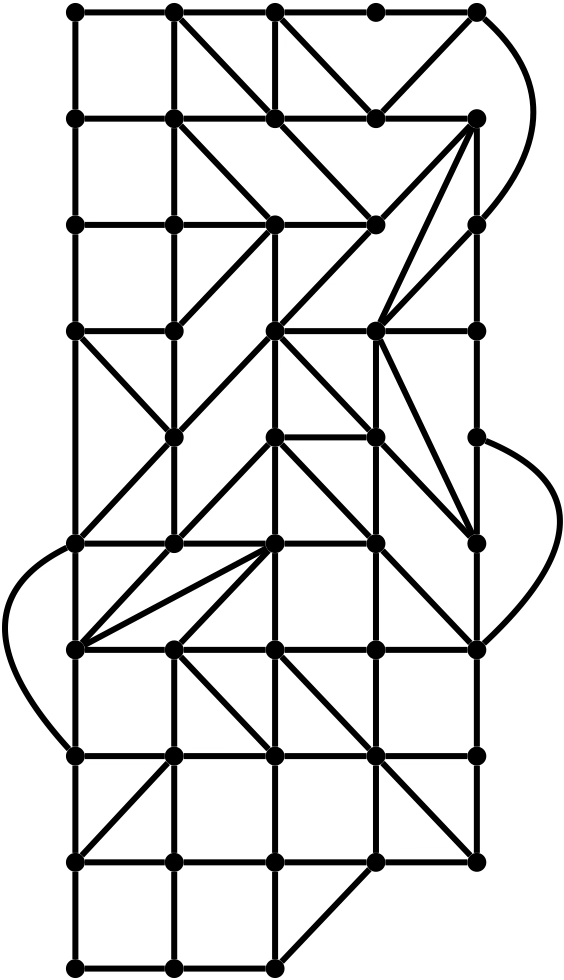
\includegraphics[width=0.6\linewidth]{../Figures/Baran-Evolving.png}
%  \caption{Baran Evolving}
%\end{marginfigure}

%Modern Clos Networks look like Decentralized Baran Networks.

%\subsection{Baran PNP}

%Partial Network Partitioning is a primary problem in the decentralized Baran Network


%\section{Baran Distributed -- Valency 4}

\marginfig[width=0.6\linewidth]{Baran-Distributed.png}[DISTRIBUTED]
 
Today's datacenter architects build their infrastructures using two kinds of boxes: \emph{switches} and \emph{servers}.

We refer to all network devices as switches. Those that route at layer 3 are simply layer 3 switches.
%\footnote{There are also many hybrid kinds of boxes, often labelled as \emph{appliances}, such as \href{http://research.google.com/pubs/pub44824.html}{load-balancers}, firewalls, etc. These are often servers in disguise.}. 
They connect them using individual cables, which they bundle together to make them convenient to route within and around physical structures. This forms a \emph{centralized} or \emph{decentralized}% \footnote{In Paul Baran's terminology (\href{http://www.rand.org/about/history/baran-list.html}{Distributed Communications}).} 
 topology, where the switches become hubs and servers become leaves.
 
\noindent \href{http://www.rand.org/about/history/baran.html}{Paul Baran's classification} %scheme 
provides insight:\\ \texttt{CENTRALIZED (A)} shows 46 univalent nodes connected to a %47$^{th}$ 
special high radix or \emph{valency}

We use \texttt{valency} to denote the number of physical ports on a hyperconverged \texttt{cell}. A \texttt{cell} is a single type of node element (autonomous unit of compute, storage and packet processing). 

A \texttt{link} is an individual, bidirectional, computation object (an autonomous communication entity between  \emph{two} \texttt{cells}) This is to distinguish us from radix, used in switches, but is equivalent to degree ($\delta$), in graph theory.

If the central hub dies, all nodes are cut off.  \texttt{DECENTRALIZED (B)} shows 47 nodes and links, 7 nodes with a valency of  5-7 serve as switches, and 40 as univalent (leaf) nodes. If one of the switches fails, the network fractures into isolated partitions; and only nodes within the partitions can continue to communicate locally. \texttt{DISTRIBUTED (C)} shows 47 identical, multivalent (valency $\sim5$) nodes, and 98 links. The network has better resilience:  failed nodes are routed around, and many links must fail before \emph{any} node is finally isolated.

%How did we get into this mess?  TCP hides so much. 
%\subsection*{Desirable \& Undesirable Topologies}
\subsection*{Datacenter Topologies}
%We all know that 
\texttt{CENTRALIZED} topologies are avoided because they represent bottlenecks and have a single point of failure. %  (SPoF's). %, so lets not talk about them anymore. 
\texttt{DECENTRALIZED} topologies are (hub \& spoke) topologies may be economically necessary for large-scale geographically disparate systems like the interstate roadways and airline networks. are  
most prevalent,  which is surprising given how \emph{non-optimal} they are  when looked at
from a perspective of distributed microservices container life-cycles

 Distributed microservices have an overwhelming predominance of East-West Traffic.  Containers can be created in microseconds and last only seconds or milliseconds.
 

 
\marginfig{Baran-redundancy.pdf}[Baran: Definition of Redundancy Level]

\marginfig{Baran-stations.pdf}[Baran: Array of Stations]
 
 
 %migration, elasticity and resilience

Today's datacenter networks evolved from their roots in the ad-hoc connection of Ethernet broadcast domains with switches housed in wiring closets and managed by individuals with specialized expertise in routing and proprietary management interfaces.

 The SPoF's in decentralized topologies are mitigated by redundancy in modern multi-slice Clos Networks. Modern Clos networks typically have two, three or four \emph{slices} of spline and leaf switches, along with multiple sets of cables..
Switches  networks that perpetuate this model, are embarrassingly complex, unreliable, arcane, and parochial. This results in very high operational costs, poor security/high vulnerability, and nothing close to five nines reliability
 [{From \href{https://www.linkedin.com/pulse/why-network-industry-has-been-stuck-1980s-ciscos-embrace-joe-howard}{Joe Howard}, The perpetuation of complexity:
 
 
\begin{quotation}
\noindent  ``Ethernet and IP networking is embarrassingly complex, unreliable, arcane, and parochial. That results in very high operational costs, poor security/high vulnerability, and nothing close to five nines reliability. In almost any other product category this would be considered unacceptable. Network technology has changed very little since the late 1980s, with the exception of faster speeds/feeds and some additional protocols and features.''
\end{quotation}}

% In almost any other product category this would be considered unacceptable. %Network technology has changed very little since the late 1980s, with the exception of faster speeds/feeds and some additional protocols and features.''
%
\texttt{DISTRIBUTED} topologies are rarely used (so far) in datacenters, except for a few HPC applications. Except for HPC applications, which have used various forms of hypercube routing, based on a cartesian coordinate system of destination addresses (a God's-Eye-View), which assumes that failures are rare, and uses complex band-aids to route around failed nodes. 

When we use a \emph{relative} addressing scheme instead, routing around failed nodes becomes far simpler, and we can build entirely new kinds of stacked graph covers to provide functionality not previously needed (or envisaged) on hypercube interconnects.. 

However, within the same \emph{or lower} capital~cost, \texttt{DISTRIBUTED} topologies provide: greater resilience, lower latencies, higher available bandwidth and far more flexibility; by connecting \texttt{cells}

We combine switches and servers, into a single concept:  \texttt{cells}, and make them \emph{substitutable (i.e. although they may not be identical in all aspects of their capabilities, they can at least be managed as one `type'.), which, in turn, makes them \emph{fungible}, and easier to manage. The additional density of the physical topology, afforded by the \texttt{cell}'s  `middle' range valency ($5$ to $9$), enables far richer virtual topologies to be built.} directly with neighbor to neighbor (N2N) %or directly-connected arrangement
connections rather than through a switched or \href{http://www.plexxi.com/2013/07/the-problem-with-everything-in-aggregation/}{aggregated} network. By not perpetuating the management complexity of switched networks, and introducing new, simpler, control/forwarding planes through \texttt{cells}, we can also dramatically lower  operational costs. 

%\footnote{This allows us to avoid almost all the problems of todays networks caused by the \href{http://www.plexxi.com/2013/07/the-problem-with-everything-in-aggregation/}{\emph{aggregation mindset}}. Just as with the naysayers in Paul Baran's time, skeptics today will often invoke \emph{argumentum ad ignorantium} (arguing that a proposition is true because it has not yet been proven false (or vice versa).  When pressed they will often fall back to the argument that: ``we've always done it this way'', or, ``it must be legacy compatible'', etc.  We contend that modern datacenter networks can gain significant advantages by adopting Paul Baran's \emph{fully distributed} model. This may not have been obvious in the past because networks were relatively static, and security was not considered a particularly important problem.}. 
% Dense networks represent an opportunity that has so far been overlooked by datacenter architects.


%Additional state stacked on top of the  \texttt{links} in TRAPHs are lost, or at least made so \emph{uncertain} we have to start again from scratch to rebuild them. Applications have to watch out for themselves, networks don't persist state. This forces ALL communications into the \emph{list} model instead of the \emph{graph} model. TRAPHs are thwarted at every turn; any graph structures they build are demolished every time a switch hiccups. %burps, farts or shits itself.

\begin{highlightbox}
\noindent Perhaps the time has come to recognize the genius of Paul Baran's insights, and ask why \texttt{DISTRIBUTED} topologies are not deployed in datacenters, where their resilience and security can be readily exploited?
\end{highlightbox}

\subsection*{Datacenter Programmability}

Two types of teams co-evolved to manage modern datacenters: one to design and manage the networks, and one to program and manage the servers. This worked % \emph{OK}% for  years,
when datacenters had a single owner or tenant, their applications and physical infrastructure evolved slowly, and different business units could work within their own silo's. % to optimize their business purpose. 
This is no longer a viable architecture in today's highly dynamic multi-tenant datacenters.

\begin{highlightbox}
\noindent Distributed applications can no longer afford to be held back by the slow pace of networking innovation.
\end{highlightbox}
% FROM ALAN: I don't see how distributed applications are being held back by the slow pace of network innovation.


%\subsection*{SDN: Programmable Networks}
%The industry's response %to the slow pace of networking innovation
%has been to introduce %the notion of 
%Software-Defined Networking (SDN) to  program networks. % behavior. 
%But SDN is  (a) \href{http://etherealmind.com/sdn-is-not-an-innovation-its-iteration/}{incremental} and (b) its \href{http://forum.stanford.edu/events/2016nickmckeowninfo.php}{programmability} continues to be confined to the \emph{network control plane}; which remains under the control of network owners and operators.
%
%High-performance forwarding chips based on PISA (Protocol Independent Switch Architecture)
%%\footnote{PISA is Protocol Independent, it allows \href{http://p4.org/spec/}{P4 programs} to specify forwarding behavior for packets. It is suitable for describing everything from high-performance forwarding ASICs to software switches. Field reconfigurability allows network engineers to change the way their switches process packets after they are deployed.} 
%can be programmed by the \href{http://www.sigcomm.org/sites/default/files/ccr/papers/2014/July/0000000-0000004.pdf}{P4 language}. While this is a step in the right direction, it is too low a level of programmability
%%\footnote{P4 presents a paradigm of ``programming with tables'' to developers. This paradigm is somewhat unnatural to imperative (or functional) programmers, and it takes some time to get accustomed to the abstraction. It also, occasionally, leads to awkward ways of expressing functionality [\href{http://arxiv.org/abs/1511.04985}{Paxos Made Switch-y].}}, 
%supporting the conventional notion that switches \emph{forward} packets to \emph{destination} addresses.
%
%%\footnote{In P4, programmers declare how packets are processed, and a compiler generates configurations for a protocol-independent switch or NIC. For example, network programmers can program the switch to be a top-of-rack switch, a firewall, or a load-balancer; and add features for monitoring or automatic diagnostics.}. 
%

While programmable switches may be a promising approach to improve the performance and manageability of datacenters, they are still (a)  under the control of the network owners and operators, and (b) limited by the low-level endpoint routing and packet forwarding paradigm of today's network engineering. What is needed to complete this revolution is to include the cells (agents on servers) as first class members of this set of devices which are allowed to route packets as well as process them.


\subsection*{TRAPHs: Programmable Application Topologies}
 
Critical layers are missing between applications and infrastructure: a layer which contains the evolving \emph{graph} relationships of modern microservices. A substrate that  programmers can own and manage themselves\footnote{A substrate that can work in conjunction with the simpler forwarding functions within NICs and switches}.
This provides the missing abstraction for a programmable, and deterministic-when-needed, topologies as tools and resources to the application architect. For example, application programmers can program these TRAPHs (Tree gRAPHs) using a Graph Virtual Machine (GVM) to provide services such as distributed consensus, atomic broadcast, and presence management among members of a cluster or microservice set. %We already have network nodes in hosts (e.g. vSwitches)

TRAPHs enable datacenter operators to organize \emph{graphs} of resources, managing them on trees, enabling computing on graphs. From the perspective of different vantage points, each with least-privilage\footnote{E.g. Managing realms, jurisdictions, tenants and sub-tenants as graphs instead of lists.}. They also provide developers of microservices complete freedom (within the nodes assigned to them), to programmatically determine their sub-relationships, and the protocol characteristics most needed for their applications.


\subsection*{Examples}

The advantage or using TRAPHS over a distributed network is that application developers can program their behavior instead of having to wait for permission, or suffer the externalities of the network optimizing itself without regard to the application's health. This simplifies some important use cases such as:
\begin{description}
	\item [Logical \& Virtual Segregation Planes] Enable capability-based security graphs, to provide secure containment of communication environments for multi-tenant infrastructures. E.g., exchange the management of lists (ACL's and \texttt{iptables}) by replacing them with richer and more manageable \texttt{graph equations}. Virtual Segregation Planes: graph applications: erasure coding, machine learning, etc.
	\item [Coherent graph overlays] where cache \emph{heterarchies} co-exist to automatically manage the placement and eviction of caches based on request patterns. One use case would be a coherent configuration file system, which provide a unified mechanism to keep configuration files synchronized, for Docker, etc. Another would be a \emph{coherent} \texttt{memcached}. Eliminating \href{https://status.cloud.google.com/incident/compute/16007?post-mortem}{cascade failure incidents}, like Google saw recently spread to all regions of their Cloud Platform due race conditions to update configuration files. 
	\item [Managing Infrastructure as Sets, Graphs \& Tensors, \emph{instead of} Boxes, Files \& Lists.]  All routing is predicated on building shortest path trees, e.g. Bellman-Ford for L2, or Dijkstra at L3. The roots for these trees are in the switches, and thus under the administrative control of network owners and operators. With TRAPHs, large subgraphs, or graph-covers comprising \texttt{cells} and \texttt{links} allocated to a particular tenant, may be used by that tenant for any topology whatsoever, including allocation to sub-tenants. \emph{Graph computing} on TRAPHs (Tree-gRAPHs) enable automatic mapping of the natural DAG relationships of distributed applications on  nested % (physical, logical, virtual)
datacenter infrastructure resources.
\end{description}

\begin{highlightbox}
\noindent \textbf{Conclusion:} Allowing application developers to build and manage their own routing substrate under API control would dramatically improve the performance, efficiency and flexibility of modern   infrastructures, reducing inter-tenant interference, enabling privacy, and improving manageability.
\end{highlightbox}

%Allowing application developers to participate in the setup and tear-down of dynamic topologies, would result is a datacenter fabric that is simpler, more resilient, easier to manage, lower cost, more secure and fundamentally more recoverable.
 
\section{The Evolution of Baran to Chiplets}

\marginfig[width=0.6\linewidth]{Baran-Decentralized-PNP.png}[Partial Network Partitioning]

\marginfig[width=0.6\linewidth]{Baran-valency-8.png}[Distributed (valency 8)]
  
\section{Baran Distributed}

\section{Baran Chiplet}

\marginfig[width=0.6\linewidth]{Baran-Chiplet.png}[Baran Chiplet]
%\end{document}


%  ladder diagram that outlines the flow of information? 

%\newpage
%\theendnotes


%%\input{TRAPH}
%[Eliminate Unnecessary Contention] e.g.  The \href{http://ieeexplore.ieee.org/xpl/articleDetails.jsp?reload=true&arnumber=6762979&abstractAccess=no&userType=inst}{TCP incast Problem}\footnote{See: http://www.pdl.cmu.edu/Incast/}. 
%\noindent Our goal is a fundamental redesign of datacenter fabrics. ; 

%Key innovations include a \emph{logical control plane} (to enhance manageability), \emph{serialization foci} (to enhance resilience and serializability), and a \emph{virtual data plane} with an integrated
 % \texttt{crdt}'s 
%\emph{metadata tensor} (to enhance consistency and recoverability); all based on a significantly improved \emph{model of time} which enables a dynamically deterministic ordering of events as a controllable (programmable) resource for distributed systems services supporting consistency, coherence, consensus and recovery.

%We seek to address fundamental customer pain points in resilience, security and manageability of \emph{configuration data} (little data) as systems scale, from the small, to the very large. Our plan is to introduce three compact low level mechanisms that enable distributed systems to be deployed quickly and easily on virtual infrastructure, and most importantly, have fast recovery capabilities in the face of perturbations (reconfigurations, failures, disasters, attacks): %Our vision is an open platform for graph computing. Our target market is cyber-defense.  For datacenters of all varieties and scales, everywhere.
%RAFE (Reliable Address-Free Ethernet ),  (AIT) Atomic Information Transfer and TRAPHs (Tree gRAPHs).


% \href{http://packetpushers.net/the-sad-state-of-data-center-networking/}{The sad state of datacenter networking.}

%\end{document}
%\clearpage
%\section*{Additional (unformatted) notes}

% Notes from Cumulus Seminar. 

%\subsection{Bridging}




\section{Transition to Layer 3-Centric Datacenter Design}

Modern datacenter network architectures are increasingly gravitating toward Layer 3 (L3) routing as the default mode of operation. While Layer 2 (L2) bridging continues to underpin legacy assumptions in application design, new trends in silicon, open networking, and container orchestration are enabling a scalable, routed foundation across the fabric.

\subsection{The Fall of Bridging: Application-Layer Assumptions}

While the network core transitions to L3, many application-level constructs still implicitly assume bridging:

\begin{itemize}
  \item \textbf{Service and Node Discovery:} Often rely on broadcast, assuming a shared subnet.
  \item \textbf{Cluster Heartbeats:} Use multicast within a broadcast domain.
  \item \textbf{VM Mobility:} Presumes persistent MAC/IP identity and L2 reachability.
\end{itemize}

These patterns constrain scalability and impede network abstraction.

\subsection{Historical Impediments to L3 Adoption}

Legacy resistance to L3 stemmed from:

\begin{itemize}
  \item Cost: Vendors historically charged premiums for L3 features and protocols (e.g., BGP).
  \item Complexity: L3 routing was perceived as difficult to configure.
  \item Lack of Host Support: Quality routing protocol stacks were unavailable on servers.
\end{itemize}

These constraints are no longer valid.

\subsection{New Enablers for Routed Datacenters}

\begin{itemize}
  \item \textbf{Merchant Silicon:} Broadcom, Cavium, and Mellanox now offer chips with bridging and routing parity in performance and cost.
  \item \textbf{Open Networking OSes:} Solutions like Cumulus Linux support native routing (e.g., Quagga, BIRD, ExaBGP).
  \item \textbf{Windows Server Support:} Native BGP support since 2012.
  \item \textbf{Routing Protocol Advances:} BGP and OSPF unnumbered simplify configuration.
\end{itemize}

\subsection{Kubernetes and the L3 Application Model}

Kubernetes abstracts applications from machines, embracing declarative scheduling and management. Key primitives:

\begin{itemize}
  \item \textbf{Pods:} Collections of containers with shared network/storage context.
  \item \textbf{Services:} Logical groups of pods, accessed via virtual IPs.
  \item \textbf{Namespaces:} Logical partitioning for policy and resource isolation.
  \item \textbf{Replication Controllers / Deployments:} Maintain pod count and manage rolling updates.
\end{itemize}

\subsection*{Networking Model}

Kubernetes defines a simple yet powerful networking model:

\begin{itemize}
  \item Every pod receives a routable IP address.
  \item Pods can communicate without NAT, even across nodes.
  \item Eliminates port mapping and collisions.
  \item Designed to operate over routed L3 fabrics (underlay or overlay).
\end{itemize}

\paragraph{Overlay Concerns:} While overlays (e.g., VXLAN) enable flexibility, they often incur significant performance overhead. Thus, L3-underlay models are gaining traction.

\subsection{Security and Isolation}

Network policy engines (e.g., Calico) leverage namespaces and DAG-style app definitions to:

\begin{itemize}
  \item Restrict Pod-to-Pod traffic
  \item Isolate workloads by namespace
  \item Enforce policy using CNI plugins
\end{itemize}

\subsection{Routing on the Host}

Hosts can participate in the routed fabric via:

\begin{itemize}
  \item \textbf{BGP Config:}
\begin{verbatim}
router bgp 65534
  bgp router-id 10.10.1.1
  neighbor eth0 interface remote-as external
  redistribute connected
\end{verbatim}
  \item \textbf{Dynamic Peering:} Using BGP unnumbered or listen range.
  \item \textbf{Stub Behavior:} Hosts are always endpoints; never transit.
\end{itemize}

\subsection{Services and Load Balancing}

\begin{itemize}
  \item Kube-proxy programs iptables to load balance across pod backends.
  \item Services expose a stable VIP, accessed via DNS.
  \item External access enabled via \texttt{NodePort} or external load balancers.
\end{itemize}

\subsection{Conclusion}

The shift from L2 bridging to L3 routing in datacenters is well underway, driven by better silicon, open software, and container-native thinking. Kubernetes exemplifies how scalable infrastructure is no longer tethered to subnet-level assumptions, and instead embraces IP-based identity, network policy, and declarative automation.

%\clearpage
%
%\subsection*{Notes for Bill Vass}
%\begin{verbatim}
% Notes for Bill Vass
%	Two pager: pains and gains
% 	Key concerns:  Cost, Reliability (of the whole stack),,  Scalability,  OPEX.
%		FOCUS on plumbing -- network switches.
%	High Level, diagram(s)
%		Reliability
%		Scalabiltiy
%		Security
%		Data Transactions  (Massive Databases)
%
%	COST
%	Resiliency
%	Ability to provide low-cost storage.  Deliver more to more customers, at higher performance and lower cost.
%	
%		What will grow his business ?
%		What keeps everyone jumping on board @ Amazon
%		Keeping client customers happy
%			Secure, data, interconnect  (Ex Baracuda)
%		Network security @ NSA
%		Deliver more with less.
%\end{verbatim}


%The \emph{shared state} becomes a resource to facilitate recovery: dedicated to re-establishing communication, and when it heals, we carry on. If that \texttt{link} doesn't heal, the \emph{shared state} (atomic tokens) are preserved and returned back to the initiator. % on the next failover tree, %stitching the \texttt{link} \emph{shared state} back together again \emph{deterministically}.  %This recovery property can be composed into any arbitrary structures stacked on top. % of those links by any number of trees. % This is TRAPHs.

%	Bill C / Al S   1/2 page Pains & Gains then next level deep
% 	Go back to Paul Baran - time to bring all that to the Datacenter, for the reasons Paul Said.
% What's different:
%	(1) a link level protocol that gives certain characteristics we can build on.
%	(2) All DC's are deploying Applications.  Applications have structure, that structure can be deployed on top of this new architecture (with N2N links). so it can be deployed and grow organically using migration to scale (evolve with demand).
%Its time to explore plumbing computers in racks without switches (or soft switches). What's different  is:
%
%(a)  A link level protocol that gives certain characteristics for distributed systems that we can build on.
%(b) Distributed applications have structure; that structure can be deployed on top of this new architecture (with N2N links). so it can grow organically using migration to scale (evolve with demand).
%
%This solves complexity; not by managing it, but by replacing it with simplicity.  Re-evaluating the topology of connection allows us to address the impedance mismatch between the virtual (distributed application) topology and the physical (switched network) topology.  

%
%We start with networking
%We continue with little data 
%We complete with computation graphs

\end{document}
